% Model development and optimization, hyper-parameter tuning, cross-validation, evaluation of models
\section{Model}

\subsection{Logistic Regression}

\subsection{Random Forest}

\subsection{Artificial Neural Network}

To build the artificial neural network (ANN) model, we used the Keras library in Python. We first developed a simple model without hyperparameter tuning or cross-validation using 13 neurons in the input layer for each feature, 64 neurons in the hidden layers, and one output neuron. We used the ReLU activation function for the hidden layers and the sigmoid activation function for the output neuron. We used the binary cross-entropy loss function \(-\frac{1}{n}\sum_{i=1}^{n}y_i \log (P(y_i)) + (1 - y_i) \log (1 - P(y_i))\), where \(y_i\) is the true label and \(P(y_i)\) is the predicted probability of the true label.
We used mini-batch gradient descent as the optimization technique. We trained the model for 100 epochs with a batch size of 10. However, when we examined the training and testing loss, we found that the model was greatly overfitting the training data, as seen in Fig.~\ref{fig:annoverfitting}. 

\begin{figure}[htbp]
    \centerline{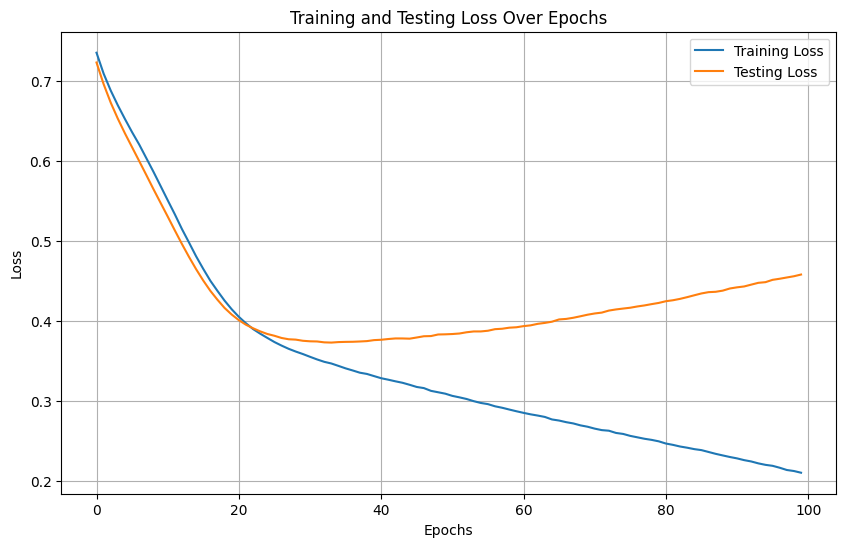
\includegraphics[width=0.7\columnwidth]{img/annoverfitting.png}}
    \caption{Training and testing loss of the simple ANN model.}\label{annoverfitting}
\end{figure}

To address this issue, we added 5-fold cross-validation and hyperparameter tuning, with dropout and momentum added. We used the GridSearchCV function from the scikit-learn library to perform a grid search over different values for the number of hidden layers (1, 2, 3), the number of neurons in each hidden layer (32, 64, 128), the dropout rate (0.1, 0.3) and the momentum term (0.5, 0.9). To further prevent overfitting and to reduce computation time, we reduced the number of epochs the model was trained for from 100 to 50. We found that the best model had three hidden layers with 128 neurons each, with a dropout rate of 0.3 and momentum term of 0.5. The best model achieved an accuracy of 0.91 on the test set, which was a significant improvement over the simple model which had an accuracy of 0.85. The confusion matrix for the best model is shown in Fig.~\ref{fig:annconfusion}.

\begin{figure}[htbp]
    \centerline{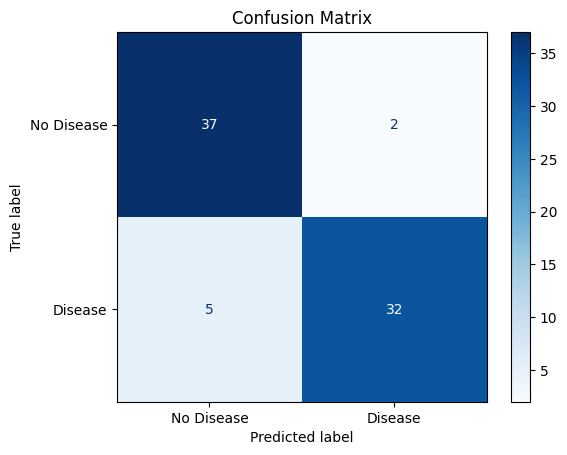
\includegraphics[width=0.7\columnwidth]{img/annconfusion.png}}
    \caption{Confusion matrix of the best ANN model.}\label{annconfusion}
\end{figure}

\subsection{Model Comparison}